\documentclass[sigconf]{acmart}

\usepackage{booktabs} % For formal tables

\usepackage{booktabs} % For formal tables
\usepackage[utf8]{inputenc}
\usepackage[spanish]{babel}
\usepackage{courier}
%\acmPrice{15.00}

% The next six lines come directly from the completed rights form.
% You MUST replace them with the lines specific to your accepted work.
\copyrightyear{2020}
\acmYear{2020}
\setcopyright{rightsretained}
\acmConference{Conference Name}{Conference Date and Year}{Conference Location}
\acmDOI{10.1145/8888888.7777777}
\acmISBN{978-1-4503-1234-5/17/07}

% Use the "authoryear" citation style, and make sure citations are in [square brackets].
\citestyle{acmauthoryear}
\setcitestyle{square}

% A useful command for controlling the number of authors per row.
% The default value of "authorsperrow" is 2.
\settopmatter{authorsperrow=4}

% end of preamble.

\begin{document}

\title{EDA y Comparación de algrotimos de ML para predecir cancelaciones en reservaciones de Hotel }

% Authors.
\author{Juan Luis Ruiz Vanegas}
\affiliation{%
  \department{Estudiante de la licenciatura en Tecnoligías para la Información en Ciencias}
  \institution{ENES, Unidad Morelia}}
\email{juanluisruiz971@gmail.com}

\author{Fernando Rodrigo Aguilar Javier}
\affiliation{%
  \institution{LTIC, ENES Morelia, UNAM}}
\email{faguilar@comunidad.unam.mx}

% This command defines the author string for running heads.
\renewcommand{\shortauthors}{Luis Ruiz, Faguilar}

% abstract
\begin{abstract}
Cómo proyecto final se pretende predecir cancelaciones en reservaciones de Hotel usando arboles de decision y regresion logistica como clasificadores.

Se pretende a su vez llevar a cabo una comparación de estos modelos de aprendizaje supervisado.

Nuestro conjunto de datos contiene información de reservaciones para hoteles citadinos y hoteles resort, además nos provee información de cuando se hizo la reservación, duración de la estadia, el número de adultos y niños, entre otros campos.

\end{abstract}

%CCS
\begin{CCSXML}
<ccs2012>
<concept>
<concept_id>10010147.10010371.10010372</concept_id>
<concept_desc>Computing methodologies~Rendering</concept_desc>
<concept_significance>500</concept_significance>
</concept>
<concept>
<concept_id>10010147.10010371.10010372.10010374</concept_id>
<concept_desc>Computing methodologies~Ray tracing</concept_desc>
<concept_significance>500</concept_significance>
</concept>
</ccs2012>
\end{CCSXML}

\ccsdesc[500]{Computing methodologies~Rendering}
\ccsdesc[500]{Computing methodologies~Ray tracing}

%keywords
\keywords{Árboles de Decisión, ...}

% A "teaser" figure, centered below the title and authors and above the body of the work.
\begin{teaserfigure}
  \centering
  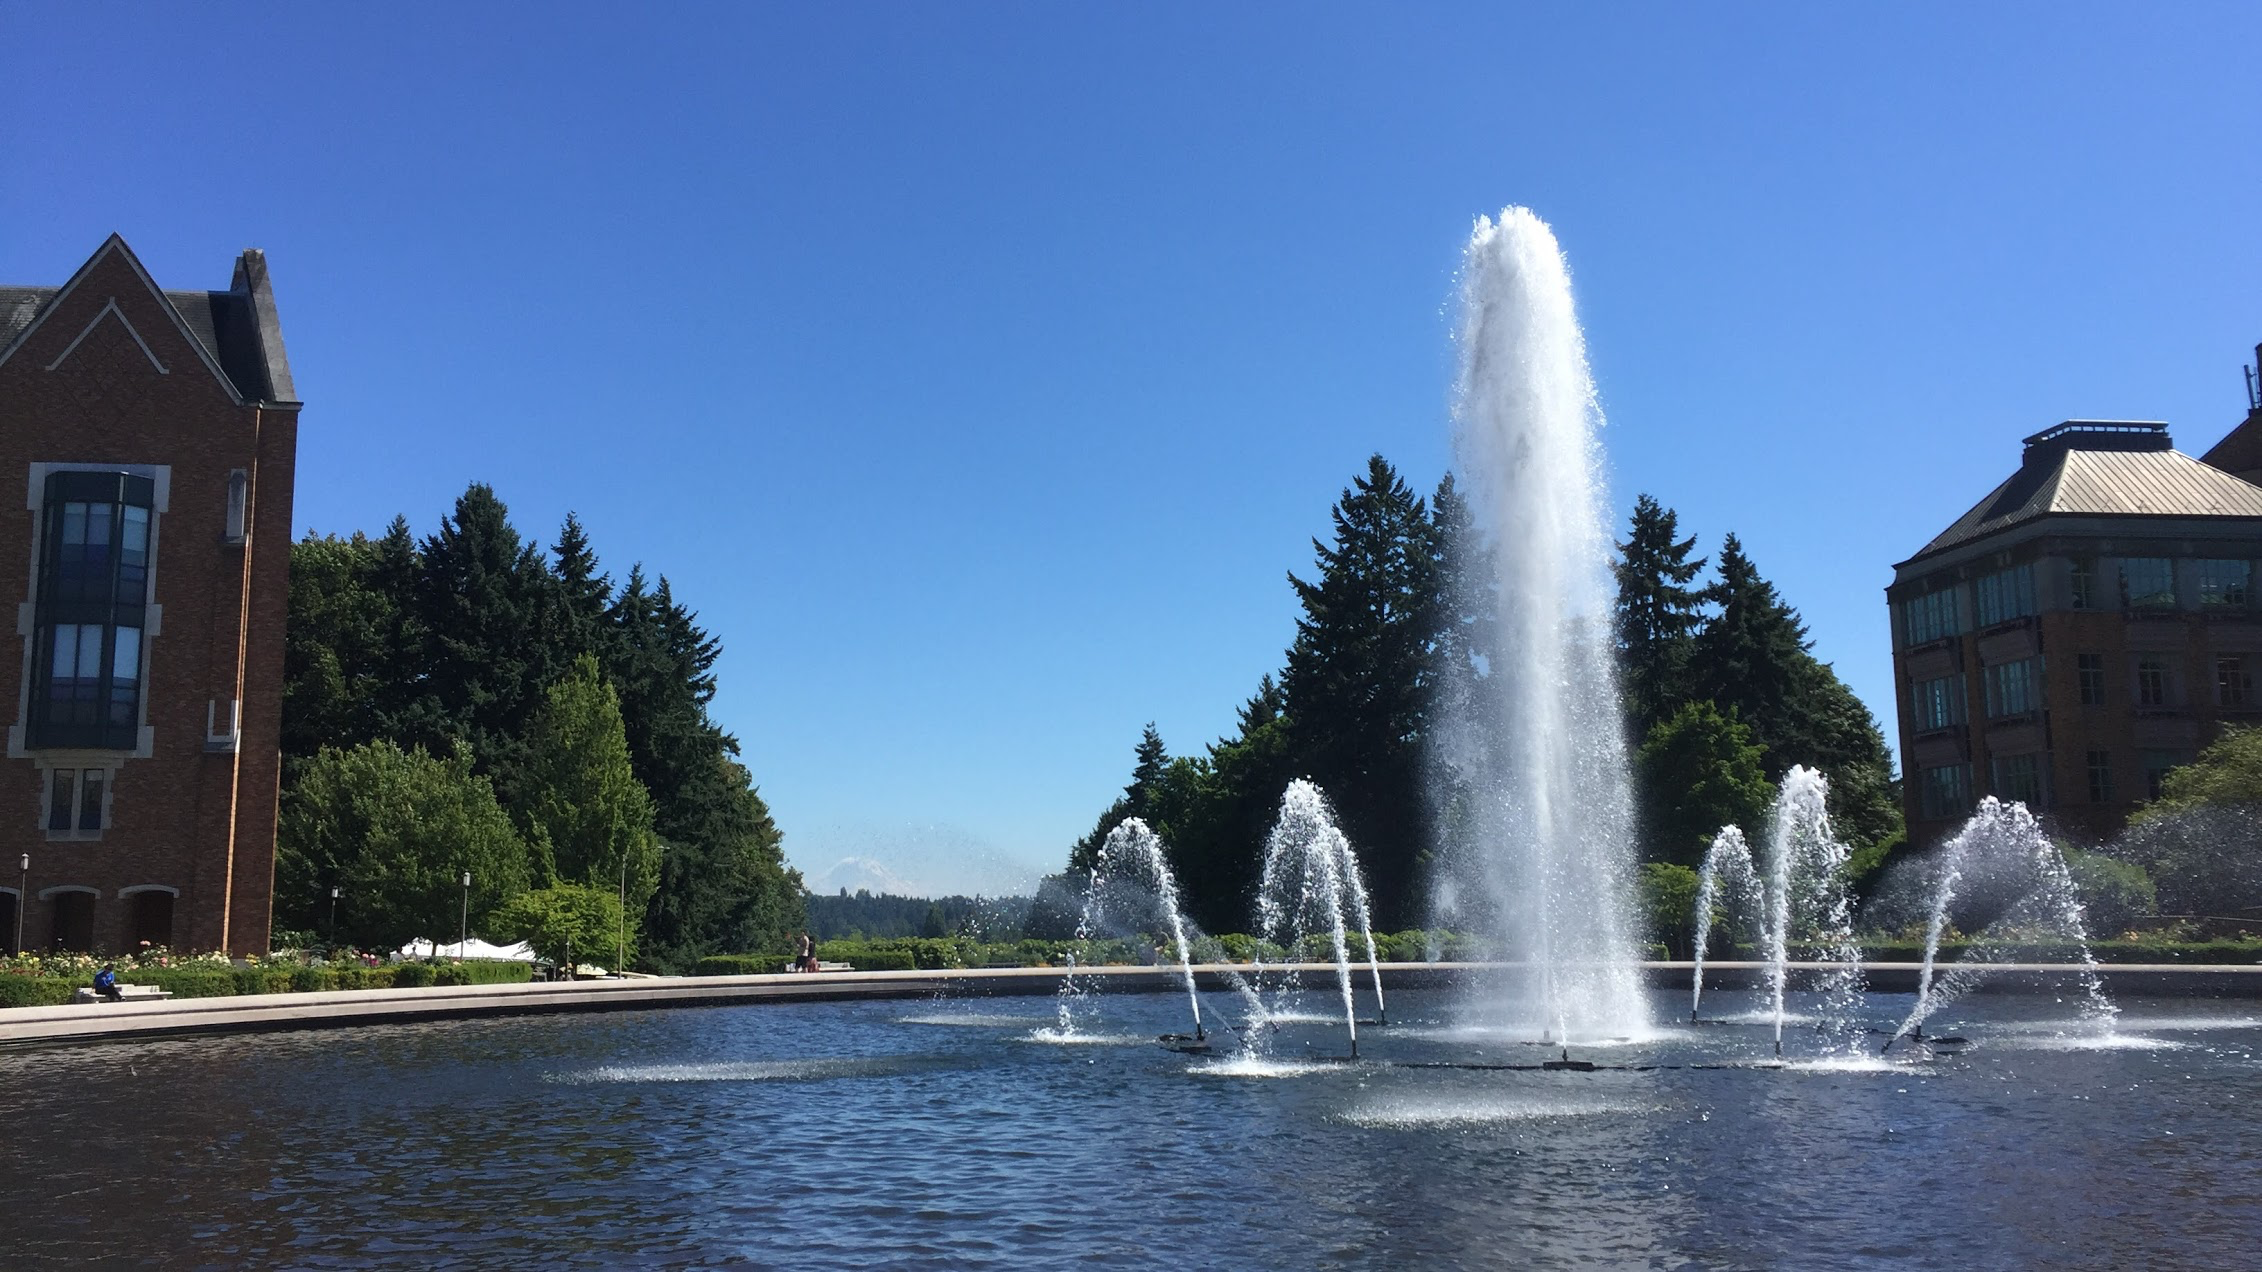
\includegraphics[width=6.0in]{aaafiles/fountain}
  \caption{Drumheller Fountain, The University of Washington, Seattle WA.}
\end{teaserfigure}

% Processes all of the front-end information and starts the body of the work.
\maketitle

\end{document}